\documentclass[tikz]{standalone}
\usepackage{tikz}
\usetikzlibrary{arrows.meta,positioning,shapes.geometric,fit,backgrounds}
\begin{document}
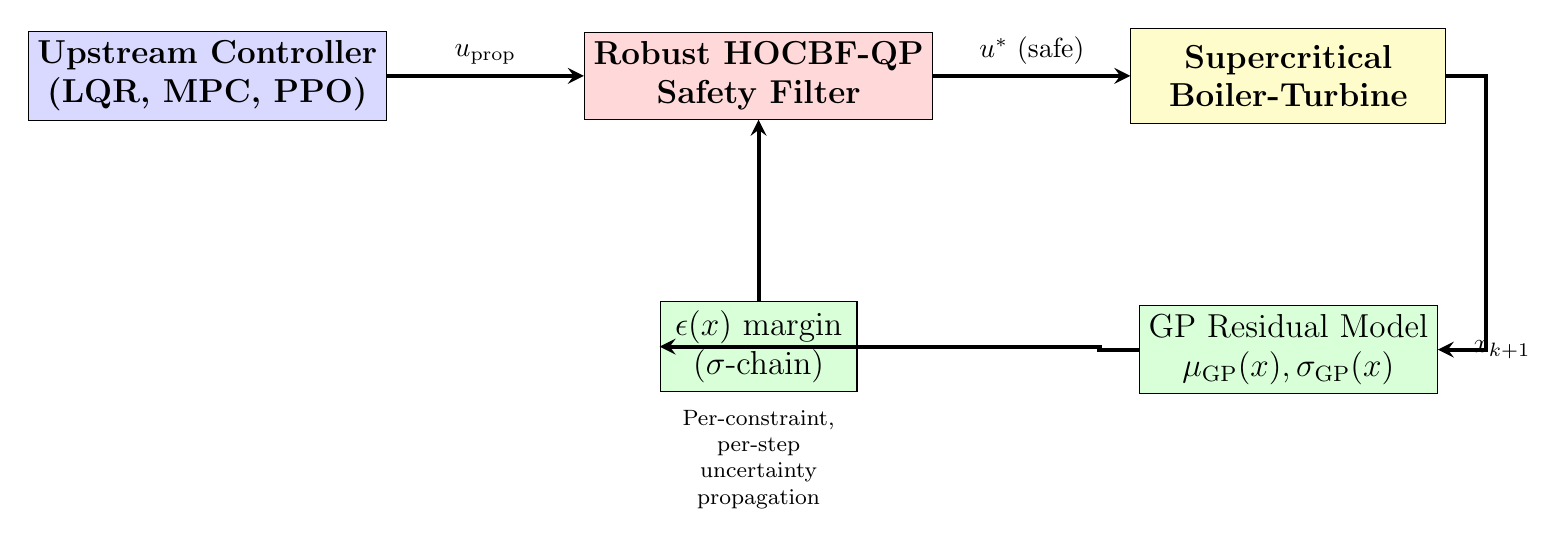
\begin{tikzpicture}[
    node distance=2.0cm,
    box/.style={rectangle, draw=black, fill=blue!15, minimum width=3.0cm, minimum height=1.0cm, align=center, font=\large\bfseries},
    gpbox/.style={rectangle, draw=black, fill=green!15, minimum width=3.0cm, minimum height=1.0cm, align=center, font=\large},
    qpbox/.style={rectangle, draw=black, fill=red!15, minimum width=3.5cm, minimum height=1.0cm, align=center, font=\large\bfseries},
    plantbox/.style={rectangle, draw=black, fill=yellow!20, minimum width=4.0cm, minimum height=1.2cm, align=center, font=\large\bfseries},
    arrow/.style={->, >=stealth, thick, line width=1.5pt}
]
    \node[box] (controller) {Upstream Controller\\(LQR, MPC, PPO)};
    \node[qpbox, right=of controller, xshift=0.5cm] (qp) {Robust HOCBF-QP\\Safety Filter};
    \node[plantbox, right=of qp, xshift=0.5cm] (plant) {Supercritical\\Boiler-Turbine};
    \node[gpbox, below=of plant, yshift=-0.3cm] (gp) {GP Residual Model\\$\mu_{\mathrm{GP}}(x), \sigma_{\mathrm{GP}}(x)$};
    \node[gpbox, below=of qp, yshift=-0.3cm, minimum width=2.5cm] (epsilon) {$\epsilon(x)$ margin\\($\sigma$-chain)};

    \draw[arrow] (controller) -- (qp) node[midway, above] {$u_{\mathrm{prop}}$};
    \draw[arrow] (qp) -- (plant) node[midway, above] {$u^*$ (safe)};
    \draw[arrow] (plant.east) -- ++(0.5,0) |- (gp.east) node[near end, right] {$x_{k+1}$};
    \draw[arrow] (gp.west) -- ++(-0.5,0) |- (epsilon.west);
    \draw[arrow] (epsilon.north) -- (qp.south);

    \node[font=\footnotesize, below=0.1cm of epsilon, text width=3cm, align=center] {Per-constraint, per-step\\uncertainty propagation};
\end{tikzpicture}
\end{document}
